\chapter{Architektura aplikace}\label{sec:ApplicationTechnology}

% TODO: specifikace požadavků
\section{Specifikace požadavků}

Aplikace by měla umožňovat vizualizaci a ladění regulárních výrazů.
Ladicí nástroj by měl být integrovanou součástí zvoleného vývojového prostředí.
Vizualizace stavů průchodu regulárním výrazem by měla být ve formě historie s intuitivním a interaktivním ovládáním, aby mohl programátor jednodušeji testovat regulární výrazy při vývoji JavaScriptových aplikací.
Program by měl umět zpracovávat nejzákladnější a běžně používané vzory regulárních výrazů, tak aby mohl být v praxi použitelný na reálných příkladech.
Dále by měla aplikace obsahovat následující prvky:
\begin{itemize}
	\item Lehká budoucí rozšířitelnost pro další možné funkcionality, které lze naimplementovat.
	\item Vizualizační část aplikace by měla obsahovat možnost zadávání regulárních výrazů a textu pro následné vyhledávání.
	\item Možnost spuštění mimo vývojové prostředí Visual Studio Code.
	\item Ladící nástroj pro vizualizaci stavů.
	\item Implementaci základních vzorů regulárních výrazů.
	\item Možnost analýzy regulárních výrazů ze zdrojových kódů.
\end{itemize}

\section{Návrh aplikace}

Aplikace je členěná na tři základní knihovny, což je zřejmé na obrázku~\ref{fig:ARCH}.
Každá část má vlastní účel a jsou od sebe navzájem izolovány.

\textbf{Knihovna rozšíření pro VSCode} se stará o komunikaci s aplikačním rozhraním (API) VSCode a o řízení všeho týkajícího se rozšíření.
Tato knihovna používá webview (webové zobrazení) k vykreslování uživatelského rozhraní pomocí vizualizační knihovny.
Rozšíření VSCode v rámci webview, zobrazuje HTML soubor index.html z vizualizační knihovny.

\textbf{Vizualizační knihovna} slouží pro zobrazení zpracovávaných regulárních výrazů.
Umožňuje zadávat regulární výrazy a testovací řetězce pro následné vyhledávání zadaným výrazem.
Jedná se o komponentu, která může být spuštěná mimo rozšíření VSCode, například ve webovém prohlížeči.
Tato knihovna závisí na knihovně vyhodnocující regulární výrazy, ale na VSCode rozšíření nemá přímou závislost.

\textbf{Knihovna vyhodnocující regexy} (zkrácení slova regular expression) slouží pro zpracovávání a vyhodnocování regulárních výrazů a pro vytváření historie stavů vyhledávání.
Tato knihovna neobsahuje závislost na dvě již zmíněné knihovny, proto může být využita například jinou aplikací.
Výsledkem této knihovny je struktura vyhledávání zadaným regulárním výrazem v podobě instance třídy \textit{RegexMatch}.

Na obrázku~\ref{fig:ARCH} je viditelná závislost mezi různými částmi aplikace. 
Rovněž je zde patrná základní struktura těchto knihoven a jejich závislosti mezi sebou.
Avšak jsou zakresleny jen ty komponenty, které lze považovat za důležité. 
%Je dobré zdůraznit asynchronní komunikaci, kterou poskytuje knihovna vyhodnocující regexy.
%Tuto komunikaci lze vidět mezi komponentou Regexer a RegexVisualizer s tím, že Regexer využívá vedlejší vlákno mimo vlákno hlavní. 
%Knihovna pro vlákna Threads.js je blíže popsána v sekci~\ref{sec:USEDtech}.
%Rozšíření VSCode v rámci webview, zobrazuje HTML soubor index.html z vizualizační knihovny.
%Také rozšíření může komunikovat s touto knihovnou pomocí zpráv, pro předávání dat a pro vyvolávání událostí. 
%RegexMatch je pak využívaný vizualizační knihovnou, pro zobrazování stavů vyhledávání.

\begin{figure}[!h]
	\centering
	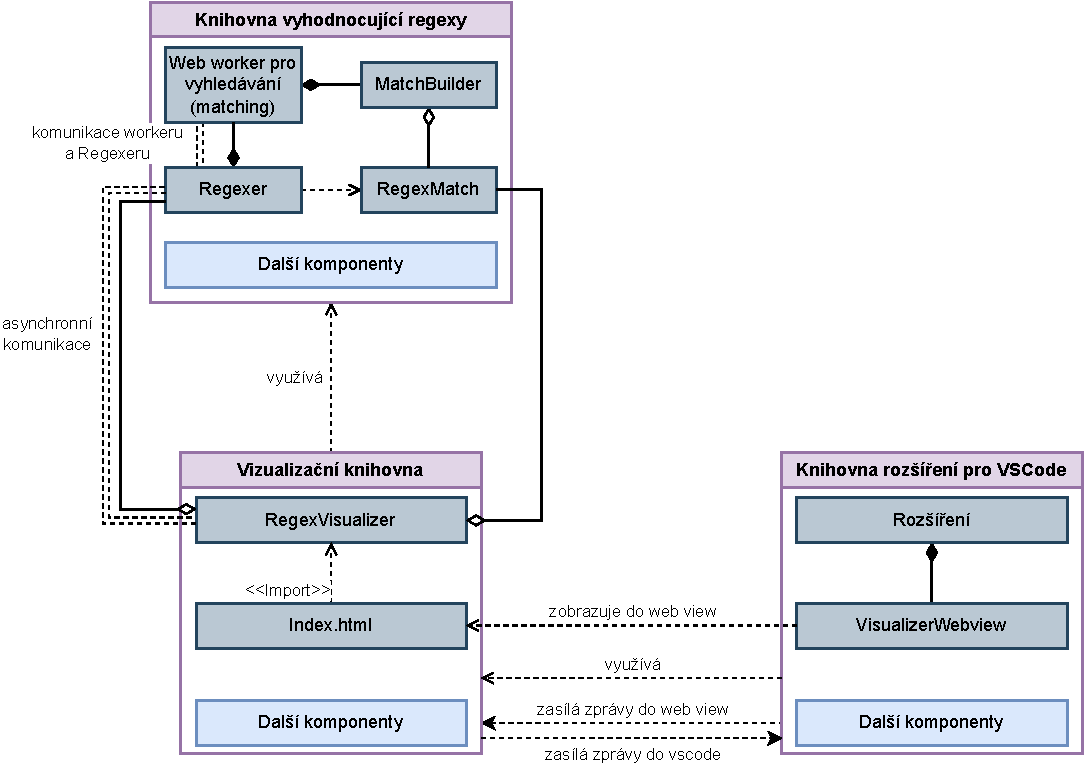
\includegraphics[width=.9\textwidth]{Figures/BP-Arch.pdf}
	\caption{Struktura knihoven aplikace}
	\label{fig:ARCH}
\end{figure}

\newpage

\section{Použité technologie}\label{sec:USEDtech}
Celá aplikace je integrovaná do vývojového prostředí \textbf{Visual Studio Code}. 
Jádro aplikace je psáno v programovacím jazyce \textbf{TypeScript} (\textit{TS}) verze 5.3, který rozšiřuje jazyk \textbf{JavaScript}, zkráceně \textit{JS}. 
TypeScript má jako hlavní nástavbu možnost využívání a přiřazování datových typů.
Psaní větší aplikace je často vhodnější v TS, kvůli svým typovým kontrolám, čímž se jako programátor mohu vyvarovat potencionálním chybám při běhu programu.
Také vývojové prostředí VSCode, zpřístupňuje API pouze pro JavaScript nebo TypeScript.
Sice by bylo možné mít část aplikace napsané v jiném jazyce, to by ale mělo své komplikace při vývoji.

Pro parsování jsem se rozhodl použít bezkontextovou gramatiku \textbf{Peggy}\cite{Peggy, Peggyjs}, pro jazyk JavaScript.
Ta umožňuje poměrně snadného zpracování textové podoby regulárních výrazů, do podoby nějaké struktury.
Tato výsledná struktura může být v podstatě jakákoliv.

Všechny části aplikace jsou spravovány balíčkovým manažerem \textbf{NPM} (Node Package Manager).
Také tyto části využívají některých balíčků, které jsou dostupné pro npm. 
Určitá část aplikace je postavená na technologii \textbf{NodeJS}.
Jedná se o JavaScript runtime (běhové prostředí), typicky určené pro serverové aplikace. 
Například runtime VSCode rozšíření je NodeJS, oproti tomu samotné webview běží ve webovém runtime, které je typické pro webové prohlížeče.

Vizualizační část aplikace pak využívá základní \textbf{HTML} (HyperText Markup Language) struktury.  
HTML je základem pro webové stránky a definuje jejich strukturu pomocí značek.
Pro následnou změnu vzhledu (stylu) jsem využil technologie \textbf{LESS}\footnote{https://lesscss.org/}, což je rozšíření standardního \textbf{CSS} (Cascading Style Sheets).
Avšak LESS musí být transpilovaný\footnote{Typ překladu z jednoho jazyka na jazyk jiný.} do CSS, jelikož webové prohlížeče ho neumí zpracovat. 
LESS umožňuje například vnořování stylů nebo tvorbu vlastních proměnných.
Pro logickou část vizualizační knihovny je také využit TypeScript.

Pro výsledný přeložený kód je použit balící nástroj \textbf{Webpack}\footnote{https://webpack.js.org/}.
Ten mi umožňuje všechny části aplikace poměrně efektivně zabalit do malého počtu souborů. 
Tento nástroj se pak hodí pro menší výslednou aplikaci a hlavně pro seskupení všech závislostí.
Mohu mít i větší kontrolu nad výsledným kódem.
Například lze udávat, kdy se mají soubory dělit, jak se mají zpracovávat přílohy, jako jsou obrázky atd.
Pro optimalizaci a úpravu kódu se zde využívá takzvaných \textit{loaderů} a \textit{pluginů}, 
které dokážou v určité části překladu zasáhnout a popřípadě změnit určitou část kódu.
Ve výsledku se jedná o velice silný nástroj, který dává programátorovi větší kontrolu nad výsledným přeloženým kódem aplikace.

Jelikož jsem chtěl mít větší jistotu, co se týče správnosti aplikace, je v algoritmické části aplikace využito technologie pro tvorbu testů. 
Tato knihovna se nazývá \textbf{Jest}\footnote{https://jestjs.io/}.
Avšak tato knihovna slouží převážně pro testování JavaScriptových kódů, proto jsem k ní využil balíčku \textbf{TS-Jest}\footnote{https://www.npmjs.com/package/ts-jest}, pro TypeScript.
To mi pak umožňuje psát testy, které mohou využívat TypeScriptové typy.

Jednou z posledních knihoven, kterou jsem použil, je \textbf{Threads.js}\footnote{https://threads.js.org/}. 
JavaScript byl navržený jako single-threaded jazyk, tudíž využití vláken, jako je známe v jiných jazycích, zde v této podobě neexistuje.
Proto existují alespoň řešení, která se snaží tuto problematiku řešit, ale neexistuje jednotná implementace pro různé runtime.
Browser má \textit{web workery} a NodeJS má \textit{worker thready}.
Sice si jsou podobné, ale mají změny, které znemožňují univerzálního použití.
Proto je v této aplikaci využito Threads.js, které eliminuje tyto problémy.
Navíc dokáže nabídnout větší bezpečnost pro programátora, který píše kód v TS. 
Tato bezpečnost je docílená tím, že knihovna dokáže poskytnout z vlákna rozhraní, které může obsahovat také typy.

\endinput